\section{Aufsetzen eines Geoservers und Einpflegen der Daten}

\subsection{Installation}

Für dieses Projekt wurde das Geoserver Projekt von der Open Source Geospatial Foundation genommen. \cite{geoserver} Dies ist ein opensoruce Geoserver der ständig gepflegt und weiterentwickelt wird. Zudem hat er eine sehr gute Documentation und eine große Community.
Desweiteren bietet er zahlreiche Erweiterungsmöglichkeiten, um zum Beispiel alle möglichen Datenquellen,Output Formate oder sonstige Services zu integrieren.

Nachdem download der aktuellsten Version, setzt man in seinem Betriebssystem den Java Pfad und den Geoserver Pfad. Dann startet man den Geoserver mit der startup Datei für sein Betriebssystem.

\subsection{Integration der Daten}

Für die Daten wurde ein eigener Workspace mit dem Namen "DeutscheBahn" eingerichtet. Unterdem dazugehörigen Verzeichnis wurden die benötigten Shapedatein hinterlegt.
Dann wurden alle Layer dem Workspace hinzugefügt. Nun ist es möglich die Layer als Preview anzeigen zu lassen.
\subsection{Methode zum Styling der Layer}

Das Styling der Layer wurde zum großteil in QGis erledigt. QGis bietet die Möglichkeit die Shapedatei hineinzuladen, ein Styling vorzunehmen und dies als ".sld"Datei zu speichern. Das Speichern funktioniert über den Stil Button.
\begin{figure}[h]
\centering
	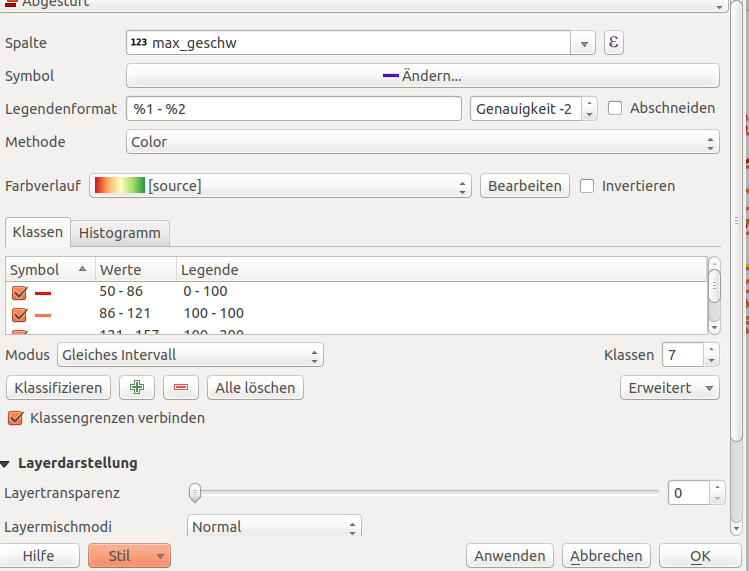
\includegraphics[width=0.5\textwidth]{images/save_styling.png}
	\caption{Abspeichern des Styling in Qgis}
\end{figure}
Dies ist ein xml Styling Format, welches das Styling eines  Layers bestimmt.
Wenn man einen Style in der Geoserver Interface erzeugt, kann man eine ".sld" Datei hochladen. Diese Datei wird einem dann in XML-Form in einem Editor dargestellt.
\begin{figure}[h]
\centering
	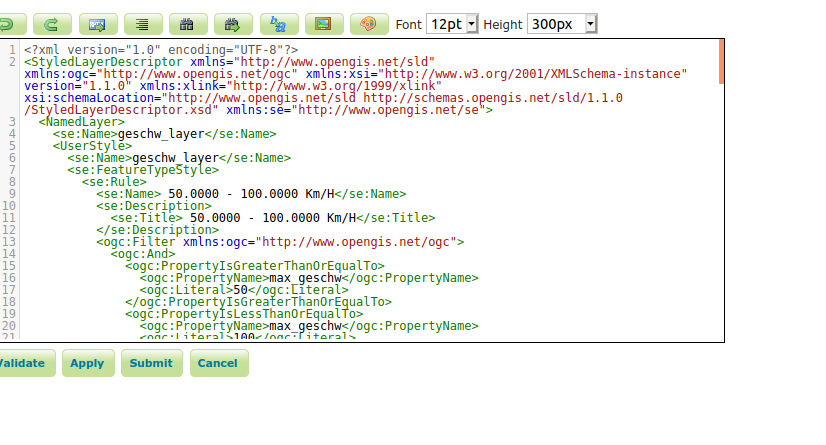
\includegraphics[width=0.5\textwidth]{images/StyleXML.png}
	\caption{XML Format der SLD-Datei}
\end{figure}
Nachdem der Style angelegt wurde, kann man in den entsprechenden Layern auf den Reiter "Publishing" gehen und das Styling als Default Styling auswählen.
\pagebreak
\subsubsection{Styling der Polygonlinien}

Das Styling der Polygonlinien in dem Projektkontext also des Schiennetz erfolgt anhand der gegebenen Attribute. Lediglich die Dicke der Linie wurde angepasst, sodass diese auch beim Reinzoomen in den Layer zu erkennen sind. Es wurde darauf geachtet, dass die Farben eindeutig zu erkennen sind. Dies bedeutet es wurde darauf geachtet kräftige Farben zu benutzen die auch beim Zoom noch zu erkennen sind.  
\begin{figure}[h]
\centering
	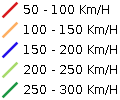
\includegraphics[width=0.3\textwidth]{images/legend_g.png}
	\caption{Legende der Geschwindigkeit}
\end{figure}
Beim Geschwindigkeitslayer war angedacht eine Abstufung vorzunehmen die von Rot was 50 Km/h bedeutet, über Gelb was der Mittelwert von 150 Km/h zu Grün was dem Wert von 300 Km/H entspricht. Das Leichtegelb war auf dem OpenstreetMap Hintergrund kaum zu erkennen und wurde dieser Farbe auf ein kräftiges Blau geändert.


Dieser Styling Vorgang wurde für die Layer Bahnnutzung,Höchstgeschwindigkeit und Elektrifizierung umgesetzt.
\pagebreak
\subsubsection{Styling der Schadstoffemissionen}
\begin{figure}[h]
\centering
	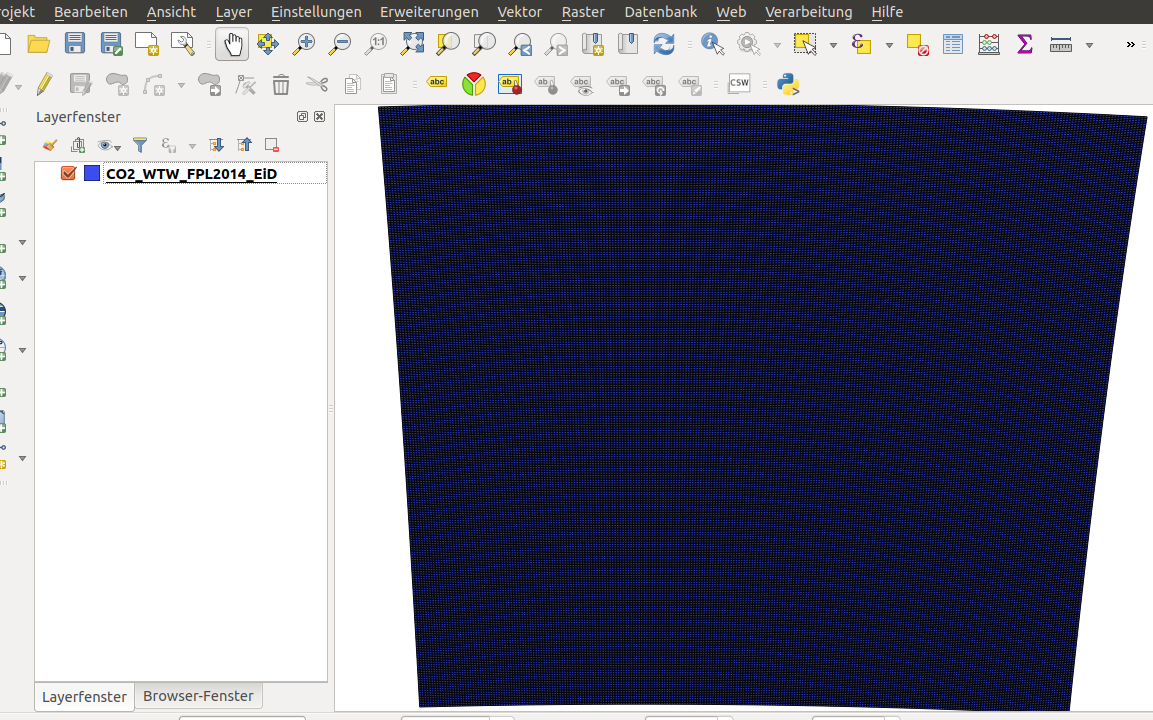
\includegraphics[width=0.5\textwidth]{images/Raster_Input.png}
	\caption{Erstes Öffnen des CO2 Shapefiles in QGis}
\end{figure}

Das Problem bei dem Styling des  Rasters war, dass jede Zelle in dem abgebildeten Raster hat einen dünnen schwarzen Rand, weshalb es auch nach Abstufung unglaublich schwer zu erkennen war wie sehr sich die Schadstoffemissionen in den jeweiligen Gebieten unterscheiden. Um viele Werte aus der Ansicht auszuschließen wurde der mindest Ausstoß(CO2 oder NOX, spielt hier keine Rolle)  pro Raster der Visualisiert werden sollten von 0 erhöht. Viele Werte innerhalb Deutschlands die eine gewisse Entfernung vom Bahnstreckennetz haben oder Werte außerhalb Deutschlands sind 0, weil dort schlichtweg keine Messwerte mit der Deutschen Bahn in Zusammenhang gebracht werden können.
\begin{figure}[h]
	\begin{subfigure}[b]{0.5\textwidth}
	\centering
	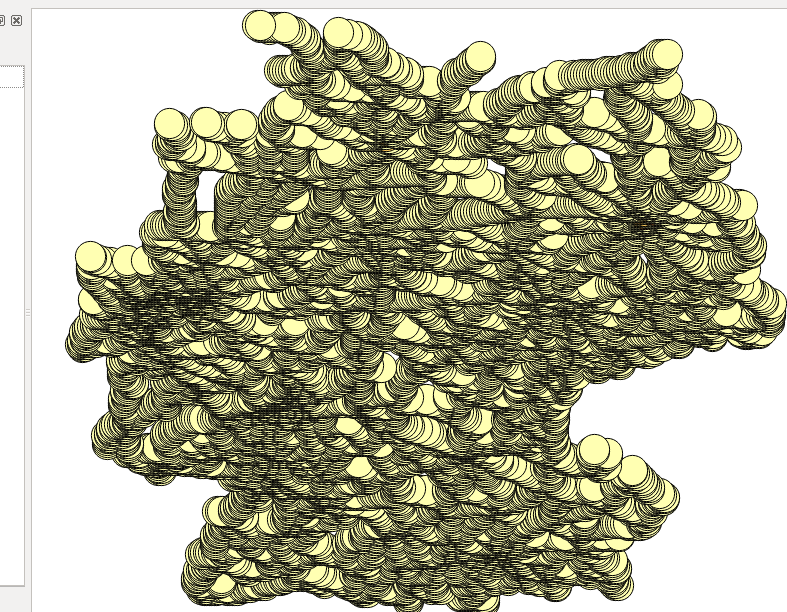
\includegraphics[width=0.8\textwidth]{images/Marker_Border.png}
	\caption{Marker with Border}
\end{subfigure}
	\begin{subfigure}[b]{0.5\textwidth}
	\centering
	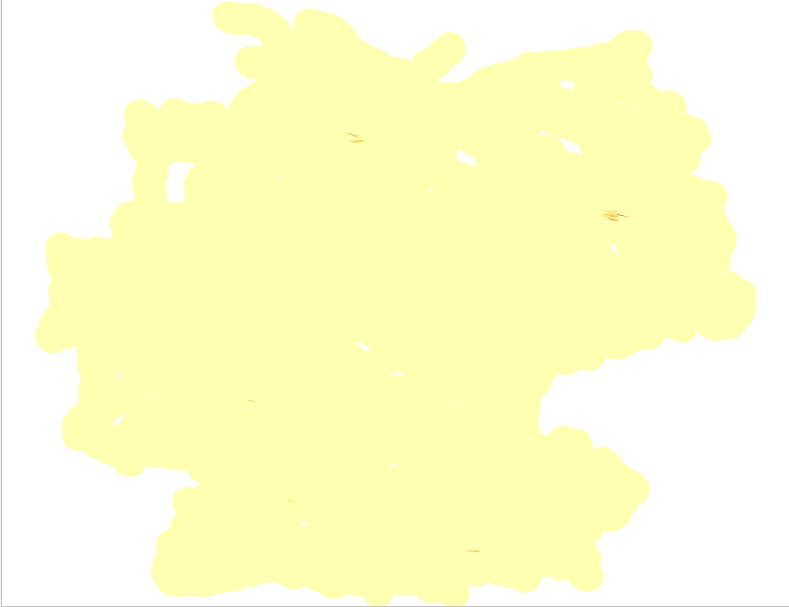
\includegraphics[width=0.8\textwidth]{images/Marker_noBorder.png}
	\caption{Marker without Border}
\end{subfigure}
\end{figure}
Die Idee ist nun eine Abstufende Farbverteilung vorzunehmen, die den jeweiligen Wert als runden Marker ohne Rand abbildet. Um die Marker auch beim Zoomen eindeutig erkennbar zu machen wurde die Größe erhöht.


Ist man weit hinausgezoomt werden die einzelnen Features übereinander gezeichnet. Dies bedeutet Features überlagern andere Features und es ist wichtig eine Reihenfolge festzulegen, sodass ein möglichst genaues Vorschaubild entsteht. In QGis gibt es nun die Möglichkeit die Zeichenreihenfolge der Features zu bestimmen. Dies erlaubt es uns erst die geringeren Werte zu zeichnen und dann die hohen Belastungswerte in kräftigem Rot darüber zu zeichnen. So ergibt sich ein sinnvolles Bild der Schadstoffbelastung in Deutschland.


\begin{figure}
\centering
	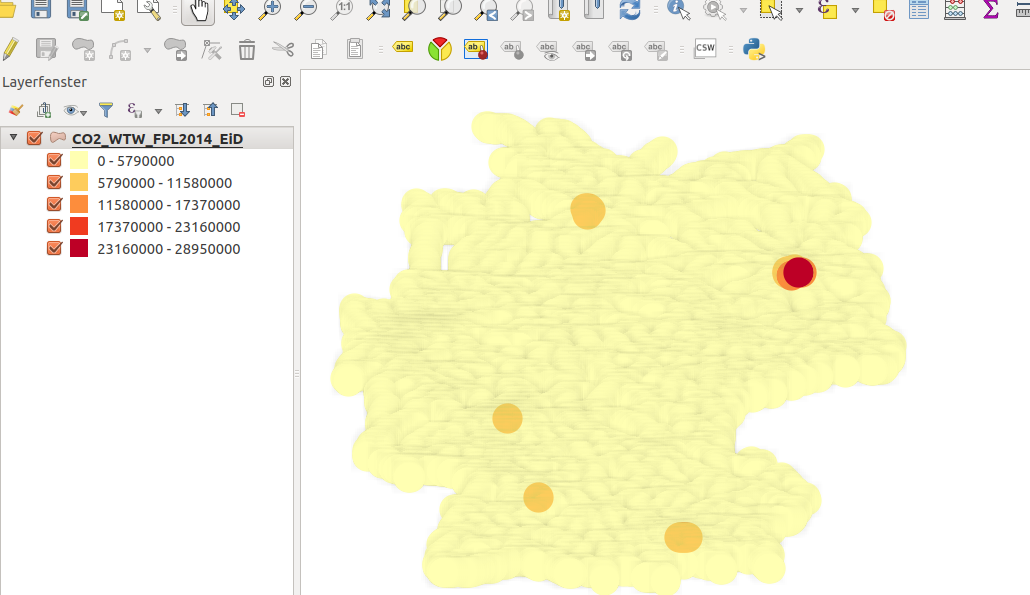
\includegraphics[width=0.5\textwidth]{images/zeichenreihenfolge.png}
	\caption{Feature Zeichenreihenfolge anhand der CO2 Belastung}
\end{figure}

Ein weiteres Problem ist, dass beim Speichern des Style in das ".sld" Format Informationen verloren gehen.

Die Stylingbeschreibung im Geoserver hatte für jedes Feature einen Randlinie und die Zeichenreihenfolge ignoriert.
Um diesen Fehler zu beheben musste man in dem XML-Editor des Geoservers die "<se:stroke" Zeile löschen die für den Rand verantwortlich ist.
Um die Zeichenreihenfolge wieder herzustellen muss die Zeile
\begin{lstlisting}
 <se:VendorOption name="sortBy">CO2kgWTW</se:VendorOption>
\end{lstlisting}
in dem FeatureTypeStyle hinzugefügt werden.
Dieser Styling Vorgang wurde für die CO2 und die NOX Belastungslayer durchgeführt.
